\documentclass{unswmaths}
\usepackage[a4paper]{geometry}
\usepackage{fancyhdr}
\usepackage{hyperref}
\pagestyle{fancy}
\begin{document}

\setlength\parindent{0pt}

\unswtitle{Adam J. Gray}{3329798}{Number Theory}{Assignment}
\fancyfoot[l]{Adam J. Gray}
\fancyfoot[r]{\today}
\fancyhead[l]{The University of New South Wales}
\fancyhead[r]{Number Theory}

\section*{Question 1}
Here is another proof that $ \sum \frac{1}{p_i} $ diverges.
For a contradiction, suppose that there is an integer $ k $ such that 
$$
	\sum_{m = k + 1}^\infty \frac{1}{p_m} < \frac{1}{2}.
$$
\subsubsection*{Part a}
Let $ p_k$ denote, as usual, denote the $ k$th  prime and let $ \alpha_k(x) $ be the number of positive integers not exceeding $ x $,
all of whose primes factors are less or equal to $ p_k $. Show that there can be no more than $2^k $ such square-free integers and then prove that $ \alpha_k(x) \leq 2^k\sqrt(x) $.
\subsubsection*{Part b}
By noting that the number of positive integers less than a given $ x $ that are divisible by the prime $ p $ is no more that $ \frac{x}{p} $, show that $ x-\alpha_k(x) < \frac{x}{2} $.
Deduce that $ x < 2^{2k + 2 } $ and arrive at a contradiction.
\subsubsection*{Solution}
\subsubsection*{Part a}
We can write every positive integer $ x $ as $ x = s^2 r $ where $ r $ is a square-free integer.  Now if we take $ x_k $ to be a positive integer whose prime factors are less than or equal
to $ p_k $, and let $ M_k $ be the set of such intengers then $ \alpha_k(x) = |M_k| $.  Writing $x_k = s_k^2 r_k $ with $ x_k \in M_k $ then each of $ p_1, \ldots, p_k $ can appear in the
 prime factorization of $ r_k $ at most once. Then there is at most $ 2^k $ ways to choose some subset of these $ k $ primes.
That is to say there there are not more than $ 2^k $ square-free integers whose prime factors are all less than of equal to $ p_k $. 

Now it also clear that there are at most $ \sqrt{x_k} $ possible
values for $ s_k $, because if $ s_k \geq \sqrt{x_k} $ then $ s_k^2 \nmid x_k $. 

This says that there are at most $ 2^k $ valid choices for $ r_k $ and at most $ \sqrt{x} $ valid choices for $ s_k $ which means that $ \alpha_k(x) = |M_k| \leq 2^k \sqrt{x} $.

\subsubsection*{Part b}
If we let $ N_{i,x} $ be the set of all integers less than or equal to $ x $ which are divisible by $ p_i $. Then let $ N_x $ be the set of all integers less than or equal to $ x $ 
which are divisible by a prime greater than $ p_k $. Then it is clear that 
$$
	N_x = \bigcup_{i=k+1}^{\infty} N_{i,x}.
$$
Now clearly $ | N_{i,x} | \leq \frac{x}{p_i} $. Note in particular that when $ p_i > x $ then $ | N_{i,x} | = 0 $. Now because $ |N_x| = x - \alpha_k(x) $ it follows that
$$ x  - \alpha_k(x) \leq \sum_{i = k + 1 }^\infty |N_{i,x}| < \sum_{i=k+1}^\infty \frac{x}{p_i}. $$
Now by the assumption laid out at the beginning 
$$ \sum_{i = k + 1}^\infty \frac{1}{p_i} < \frac{1}{2} $$ so $$ \sum_{i=k+1}^\infty \frac{x}{p_i} < \frac{x}{2} $$
and thus $ x - \alpha_k(x) < \frac{x}{2} $ or $ \alpha_{k}(x) > \frac{x}{2} $.

So we now have an upper and lower bound on $ \alpha_k(x) $ given by
$$
	\frac{x}{2} < \alpha_k(x) < \frac{2^k}{\sqrt{x}}
$$
but say $ x = 2^{2k+4} $ then $ 2^{2k+3} < \alpha_k(x) < 2^{2k+2} $ which is clearly a contradiction,
so our assumption that there exists a $ k $ such that 
$$
	\sum_{m=k+1}^\infty \frac{1}{p_m} < \frac{1}{2} 
$$
is wrong and hence $ \sum \frac{1}{p_i} $ must diverge.
\section*{Question 2}
\subsubsection*{Part a}
Show that if  $ p $ is prime and $ p | x^2 + 2 $ then $ p \equiv 1 $ or $ 3 \mod 8 $.
\subsubsection*{Part b}
By considering $ N = (p_1 \ldots p_r)^2 + 2 $, where $ p_i \equiv 3 \mod 8 $, prove 
that there are infinitely many primes congruent to $ 3 \mod 8 $.

\subsubsection*{Solution}
\subsubsection*{Part a}
This statement is actually false because $ 2 \equiv 0^2 + 2 \mod 8 $, however, for $ x > 0 $ the
statement is true.

Note that for any integer $ x $ we have that $ x^2 + 2 \equiv 2, 3, 6 \mod 8 $,
so if $ pk = x^2 + 2 $ for some integer $ k $ and prime $ p $ then we must have
$ pk \equiv 2,3,6 \mod 8 $. Clearly $ p \not\equiv 2, 6 \mod 8 $ because then $ p $ would
be divisible by $ 2 $ and hence not a prime, unless $ p = 2 $ and this case was dealt with at the start of the proof.

We are therefore left to consider the following 3 cases as such:
\begin{itemize}
	\item So if $ pk \equiv 3 \mod 8 $ then we could have $ p \equiv 1 \mod 8 $, $ k \equiv 3 \mod 8 $ or $ p \equiv 3 \mod 8 $ and $ k \equiv 1 \mod 8 $.

	\item If $ pk \equiv 2 \mod 8 $ then we could have $ p \equiv 1 \mod 8 $ and $ k \equiv 2 \mod 8 $.

	\item If $ pk \equiv 6 \mod 8 $ then we could have $ p \equiv 1 \mod 8 $, $ k \equiv 6 \mod 8 $ or $ p \equiv 3 \mod 8 $ and $ k \equiv 2 \mod 8 $.
\end{itemize}
In each case $ p \equiv 1 $ or $ 3 \mod 8 $. \qed

\subsubsection*{Part b}
Suppose there are finitely many primes of the form $ p \equiv 3 \mod 8 $. Then write $ N = (p_1\ldots p_r) + 2 $ where $ (p_1\ldots p_r) $ is the product of all such primes.
Note that $ N \equiv 3 \mod 8 $. Now consider the prime factorization of $ N = (q_1^{\alpha_1}\ldots q_j^{\alpha_j}) $. From part a we have that 
each $ q_i $ must be either $ q_i \equiv 1 $ or $ 3 \mod 8 $, but as $ N \equiv 3 \mod 8 $ there must be at least one $ q_k $ such that $ q_k \equiv 3 \mod 8 $,
but this $ q_k $ cannot appear in the product $ (p_1\ldots p_r) $ because $ (p_1\ldots p_r)^2 + 2 \mod p_i \equiv 2 \mod p_i $ for all choices of $ p_i $, 
whereas $ q_k | (p_1 \ldots p_r)^2 + 2 $. This is a contradiction because $ q_k \equiv 3 \mod 8 $ but we assumed $ (p_1 \ldots p_r) $ was the product of all $ 3 \mod 8 $ primes.
So our assumption must be wrong and there must be an infinite number of primes congruent to $ 3 \mod 8 $. \qed

\section*{Question 3}
Write $ \pi^*(x) $ for the number of integers not greater than $ x$, that are of the form $ p^k $ for some prime $ p $ and some integer $ k $. (Hence $ \pi^*(x) $ counts primes
and prime powers.)
\subsubsection*{Part a}
Explain why
$$
	\pi^*(x) = \pi(x) + \pi(x^\frac{1}{2}) + \pi(x^\frac{1}{3}) + \ldots + \pi(x^\frac{1}{m}), 
$$
where $ m $ is the largest integer such that $ 2^m \leq x $.
\subsubsection*{Part b}
Suppose $ C $ is a constant such that $ \pi(x) \leq \frac{Cx}{\log(x)} for all  x \geq 2 $.
Explain why $ \pi^*(x) - \pi(x) \leq \frac{Cx}{\log(x)} $ for all $ x \geq 2 $.
Explain why $ \pi*(x) - \pi(x) \leq \pi(x^\frac{1}{2}) + m\pi(x^\frac{1}{3})$, with $ m $ as in (a), and hence
prove that 
$$
	\pi*(x) = \pi(x) \leq 12C\frac{x^\frac{1}{2}}{\log(x)}
$$
for all $ x \geq 2 $. (Hint: the inequality $x^\frac{1}{3}\log(x) \leq 6e^{-1}x^\frac{1}{2}$ may be useful.)
\subsubsection*{Part c}
What does this tell us about prime powers? (Hint: plot $ \frac{x^\frac{1}{2}}{\log(x)} $ )
\subsubsection*{Solution}
\subsubsection*{Part a}
Note that 
\begin{align*}
	\pi(x^\frac{1}{k}) &= | \{ p : p \leq x^\frac{1}{k}, p \text{ prime } \} | \\
		&= | \{ p : p^k \leq x, p \text{ prime } \} |
\end{align*}
so clearly 
\begin{align}
	\label{q3:result}
	\pi^*(x) = \sum_{k=1}^\infty \pi(x^\frac{1}{k}) 
\end{align}
but when $ 2^m > x $ then any prime $ p $ is such that $ p^m > x $ and hence 
\begin{align*}
	\pi(x^\frac{1}{m}) &= | \{ p : p \leq x^\frac{1}{m} \} | \\
		&= | \{ p : p^k \leq x \} | \\
		&= 0
\end{align*}
and so we can rewrite \ref{q3:result} as 
\begin{align*}
	\pi^*(x) = \sum_{k=1}^{\lfloor \log_2(x) \rfloor} \pi(x^\frac{1}{k})
\end{align*}
as required.
\qed

\subsubsection*{Part b}
Let $ m = \lfloor \log_2(x) \rfloor $ as it was (implicitly) in part (a).
Then see that 
$$ 
	\pi*(x) - \pi(x) = \pi(x^\frac{1}{2}) + \underbrace{\pi(x^\frac{1}{3}) \ldots + \pi(x^\frac{1}{m})}_{m-1 \text{ terms }} 
$$
so 
\begin{align*}
	\pi^*(x) - \pi(x) &\leq \pi(x^\frac{1}{2}) + m\pi(x^\frac{1}{3}) \\
\end{align*}
and by the assumption $ \pi(x) \leq \frac{Cx}{\log(x)} $ for  all $ x > 2 $ then we have
\begin{align*}
	\pi*(x) - \pi(x) &\leq C\left( \frac{x^\frac{1}{2}}{\frac{1}{2}\log(x)} + \frac{mx^\frac{1}{3}}{\frac{1}{3}\log(x)} \right) \\
	&= C\left(\frac{2x^\frac{1}{2}}{\log(x)} - \frac{3\lfloor \log_2(x) \rfloor x^\frac{1}{3}}{\log(x)} \right) \\
	&\leq C\left(\frac{2x^\frac{1}{2}}{\log(x)} - \frac{3 \log_2(x) x^\frac{1}{3}}{\log(x)} \right) \\
	&= C\left(\frac{2x^\frac{1}{2}}{\log(x)} - \frac{3 x^\frac{1}{3}}{\log(2)} \right) \\
	&= C\left(\frac{2x^\frac{1}{2}\log(2)}{\log(x)\log(2)} - \frac{3 x^\frac{1}{3}\log(x)}{\log(2)\log(x)} \right) \\
    \text{ and by the inequality mentioned in the question we have} \\
    &\leq \frac{Cx^\frac{1}{2}}{\log(x)} \left(\frac{2+18e^{-1}}{\log(2)}\right) \\
\end{align*}
and by numerical evaluation of $ \left(\frac{2+18e^{-1}}{\log(2)}\right) \approx 12.439 $ we must have that
\begin{align*}
    \frac{Cx^\frac{1}{2}}{\log(x)} \left(\frac{2+18e^{-1}}{\log(2)}\right) \leq 12C \frac{x^\frac{1}{2}}{\log(x)}
\end{align*}
so 
$$
    \pi^*(x) - \pi(x) \leq 12C \frac{x^\frac{1}{2}}{\log(x)}.
$$
\subsubsection*{Part c}
\begin{center}
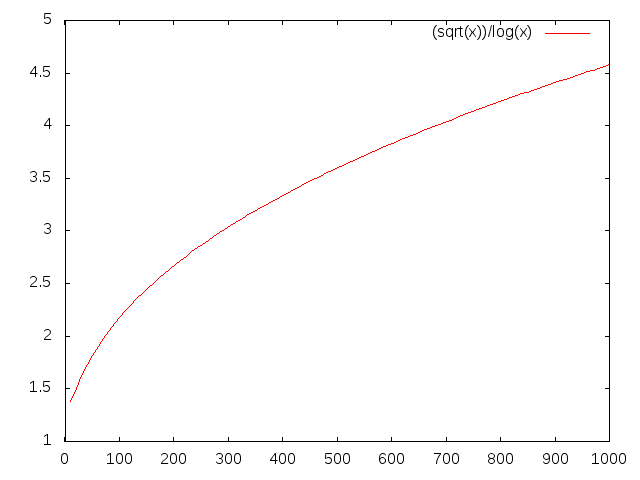
\includegraphics[scale=0.5]{plot}
\end{center}

This tells as that as $ x \longrightarrow \infty $ prime powers get ``less common'',
in particular because $$ \frac{x^\frac{1}{2}}{\log(x)} < \frac{x}{\log(x)} $$ for sufficiently
large $ x $ it tells us that in some sense prime powers are ``less common'' than primes.

\section*{Acknowledgements}
The proof from question 1 is based off a proof by Erdos, and a similar proof can be found on Wikipedia
at \url{http://en.wikipedia.org/wiki/Divergence_of_the_sum_of_the_reciprocals_of_the_primes}. This was
pointed out to me by Adrian Miranda.

\end{document}
